% !TEX root = ../main.tex


%-- number of constraints?
\chapter{Proof construction}
We will be using Circom to generate an arithmetic circuit, and SnarkJS for the proof generation.


\paragraph{Circom} is a domain-specific language for creating arithmetic circuits, which are used in zk-SNARKs.
The circuit code can be written to specify the desired constraints.
Circom allows expressing the circuit's arithmetic operations, constraints, input and output in a concise and readable manner.
Once the circuit is designed, it needs to be compiled into a format suitable for zk-SNARKs.




\paragraph{SnarkJS} is a JavaScript library that provides tools for working with zk-SNARKs, including circuit compilation.
After compilation, SnarkJS facilitates generating zk-SNARK proofs for specific instances of the circuit.
SnarkJS also provides utilities for verifying the proofs.


\section{Proof of liabilities}
\label{subsec:pl}
The proof of liabilities operates on a list of balances and a list of email hashes as private inputs.
The first purpose of the circuit is to validate that all values are non-negative and that all balances fall within a specified range.
These verifications are crucial to prevent overflow or underflow issues, given that the operations occur within a finite field.


Subsequently, the proof of liabilities constructs a Merkle tree and outputs the total balance sum and the root hash of the Merkle tree.


\paragraph{Inputs}
\begin{itemize}


   \item List of balance (private)
  
   \item List of email hash (private)
  
   \end{itemize}


\paragraph{Outputs}
\begin{itemize}
   \item Balance Sum (public)
   \item Root hash (public)
   \item No negative values (private) - boolean
   \item All small range (private) - boolean
   \end{itemize}


This proof of liabilities operates as intended because it returns the sum of the liabilities, which is exact because of the checks.
It also returns the root hash, ensuring you cannot alter any values inside the merkle tree. The merkle tree is hidden so that we do not
give any information about users and their balances.
The root hash will be used to verify the inclusion of the balances.




In a complete proof of reserves, the balance sum would be a private output. We would have another circuit proving that the sum of liabilities is smaller
than the sum of assets, without revealing the balance.




\section{Proof of inclusion}
\label{subsec:pi}
The proof of inclusion aims to prove that the balance of a user is included in the Merkle Tree created in the proof of liabilities.
To prove that a balance is included, it is sufficient to show that you know the Merkle path of a user balance,
which we define using the list of neighbors sum, hash and binary.
The neighbors binary variable indicates whether the neighbor is on the left or the right.
The root hash, root sum, user balance and user email hash are public because it needs to be shown which user is in which tree.


In figure 4.1, Charlie is defined as the user. The merkle path is composed of the three blue nodes. In each blue nodes we can find the variables of the lists,
namely the binary (left or right), the sum and the hash.
\begin{figure}[H]
   \centering
   \includegraphics[width=130mm]{MerklePath.png}
   \caption{Merkle Path \cite{BM22}}
   \label{overflow}
   \end{figure}


\paragraph{Inputs}
\begin{itemize}


   \item List of neighbors sum (private)
  
   \item List of neighbors hash (private)


   \item List of neighbors binary (private)


   \item Root hash (public)


   \item Root sum (public)


   \item User balance (public)


   \item User email hash (public)
  
   \end{itemize}


\paragraph{Outputs}
\begin{itemize}
   \item Balance included (public) - boolean
   \end{itemize}


\paragraph{}
In the circuit, we verify that the combination of the user balance, sum and merkle path gives the right root hash and root sum. There is no additional
verifications since they are already done for this root hash, in the proof of liabilities.




\section{Daily proof of liabilities}
We aim to enhance our current \hyperref[subsec:pl]{circuit} by minimizing the work needed in subsequent rounds.
The first thing to explore is recursion proofs, as they were specifically created to reduce the total computational effort across rounds.




\subsection{Aggregation proofs}
The main advantage of the aggregation proof is in streamlining the verification process. For instance, in the second round, we can prove the integrity of the current round and all previous rounds.
However, this benefit comes with trade-offs. The first drawback is the increase in proof size, as it necessitates to prove the current circuit and verify the previous ones.
When considering the frequency of verification, having a fixed number of nodes verify the proof daily, it would be illogical to make the nodes verify the previous rounds every single day.
On the other hand, if the verification is not consistent, or there is a need for new nodes to be able to come in and verify every proof quickly, then aggregation becomes more appealing.


In our case, the priority is to produce daily succinct proofs. We need to ensure the integrity of every round, while keeping the proof size to a minimum.
Therefore, having our nodes verify the circuit at every round without the computational overhead of the aggregated proof is sufficient.




\subsection{Other recursion proofs}
The aggregation proof stands out as the only recursion proof potentially useful in certain scenarios.
If we examine the other types of recursion proofs, namely Recursion scheme, accumulation and Folding scheme, they all have one thing in common.
They are all designed to verify multiple rounds concurrently.
This approach is not aligned with our objectives. We are interested in working on rounds independently and reducing the individual workload.




\subsection{New circuit}
If we cannot use any recursion schemes, we need an alternative approach to reduce the complexity of subsequent rounds.
Our solution is to reutilize the same Merkle Tree as the previous rounds, modify  and adapt it to include the changes.
The key challenge is that the Merkle Tree was built inside the circuit, and is therefore not accessible.


What we will be doing, in our modified circuit, is adjust the Merkle Tree inside the circuit.
For every change, we send the corresponding Merkle Path which will be verified by the circuit.
The circuit will then compute a new Root Hash for each change and output the final Markle Hash.



The standard verification will be applied to the new values (e.g., non-negative values, limited range).


\paragraph{Inputs}
\begin{itemize}


   \item List of old email hash (private) - 1 per change
  
   \item List of old values (private) - 1 per change


   \item List of new email hash (private) - 1 per change
  
   \item List of new values (private) - 1 per change


   \item List of temporary root hash (private) - 1 per change
  
   \item List of temporary root sum (private) - 1 per change


   \item New root hash (public)


   \item New root sum (public)


   \item Old root hash (public)


   \item Old root sum (public)


   \item List of neighbors sum (private) - 1 list per change


   \item List of neighbors hash (private) - 1 list per change


   \item List of neighbors binary (private) - 1 list per change
  
   \end{itemize}


   \paragraph{Outputs}
   \begin{itemize}
       \item Valid hash
       \item Valid sum
       \item No negative values
       \item All small range
       \end{itemize}


To recapitulate, for every change in the merkle tree, we have the merkle path with the old values, the new values, the temporary root hash and
the temporary root sum.
The merkle path is used as an inclusion proof for the old value, and is used to verify the temporary root hash.
The circuit is iterating over the changes and gives a final root hash. We verify that the final root hash and sum are the same as inputs.

\subsection{Minimizing the number of changes}
To minimize the number of constraints, we want to minimize the number of changes.
We define a change as a hash change at the bottom level. Any new user, balance change or removal of old user is considered as a change.
The naive change calculation would be $#change = #balance change + #new user + #deprecate user$.
However, a new user can take the node of a deprecater user. So we would have the equation $#change = #balance change +max(#new user + #deprecate user)$

\subsection{Constraint analysis}
Theorically, the new circuit makes sense. It should be quite faster than the old one, so let's analyze it.
First, lets look at doing a daily proof where there is a change in the user's value.

The first assumption we are gonna need to do, is to assume the number of balance change. A completely subjective number would be $1\%$.
%--first graph
Once you reach more than 128 users with $1\%$ change, it is not worth it to use the new circuit. This is not much practical.
However, we can see that the number of constraints of the new circuit grows linearly for the number of change.
Instead of looking at the changes daily, we could do it hourly.
Going with the assumption that $1\%$ change daily, we will assume that $0.05\%$ of the balances changes hourly.
Lets look at the number of constraints if $0.05\%$ of users change every hour.
%--second graph
Even with more than 1 million users, there is still 3 times less constraints with our new circuit.
So if we want to do an hourly proof, it is less expensive with the new circuit than the old circuit.
We can take this a step further, and do a proof at every new block. We could have a merkle tree up to date for the liabilities side at every single block.
While the hourly proof and block proof is better with the new circuit, maybe a daily proof is sufficient for someone.


\subsection{Folded proof of liabilities}
With the old circuit, we saw how it was not usefull to use folding or any other recursion scheme.
However, with the new circuit, we have multiple proof that we want to prove faster and verify faster.
We can separate our proof of $n$ changes into $m$ proofs, where $m <= n$, and fold the circuits together.
%--- minmax the number of fold we want (graph for 1 change, graph for 2 change, graph for 3 change)
%--- change old circuit vs new circuit (1% change) vs new folded circuit (20*0.05%)
%proof time, verifier time, proof size graph


%describe the folded circuit
%put in psuedocode of circuit
%maybe a few snipplets of real code, explaining anything that was difficult to do
%put code of proof of inclusion, proof of liabilities, and proof of liabilities change

\section{Daily proof of inclusion}


Because a marketplace can have millions of users, it is impractical to build a proof of inclusion for every single user on a daily basis.
It is the user's responsibility to request a proof that their balance is included in the published Merkle tree.


In an ideal world, a Merkle tree would be published at least daily. However, it is once again impractical to require every user to verify their inclusion everyday.
Nevertheless, each user verifying its inclusion in the tree increases the chance that the proof of liabilities is valid and includes every single balance.
This is why it is primordial to find a way to make it easier to verify the inclusion. This is where Nova folding schemes come in.


The novel way to do proof of inclusion is to generate a proof of inclusion that is valid from the day of creation of the account, to the requested day by the user.
Normally you would need to create 500 different proofs for 500 days. However, we saw in the previous section that the nova folding scheme enables the 500 proofs into just one.
Verifying this one proof is the equivalent of verifying the 500, or any other number of days required.
This drastically simplifies the verification process.


Previously, when requesting a proof of inclusion, the user would only receive proof that their balance is included in the latest published Merkle tree. Now, the proof verifies that the balance has been included in every previously published Merkle tree.
This ensures that any malicious entity would be unable to alter ownership of balances across multiple days. It might seem like a small detail, but it is the detail that makes all the difference, and here is why.


In this chart, we can observe the failure probability, which represents the likelihood that a dishonest prover gets away with misbehaving.
If we take for example the orange line, where an exchange has 1 million users, we notice that the failure probability approaches 0 when over $4\%$ of users perform their verifications.
However, without utilizing folding, this principle doesn't extend to every round. It implies that for each round, we require a minimum of $4\%$ of users to have a proof with significant confidence.


\begin{figure}[H]
   \centering
   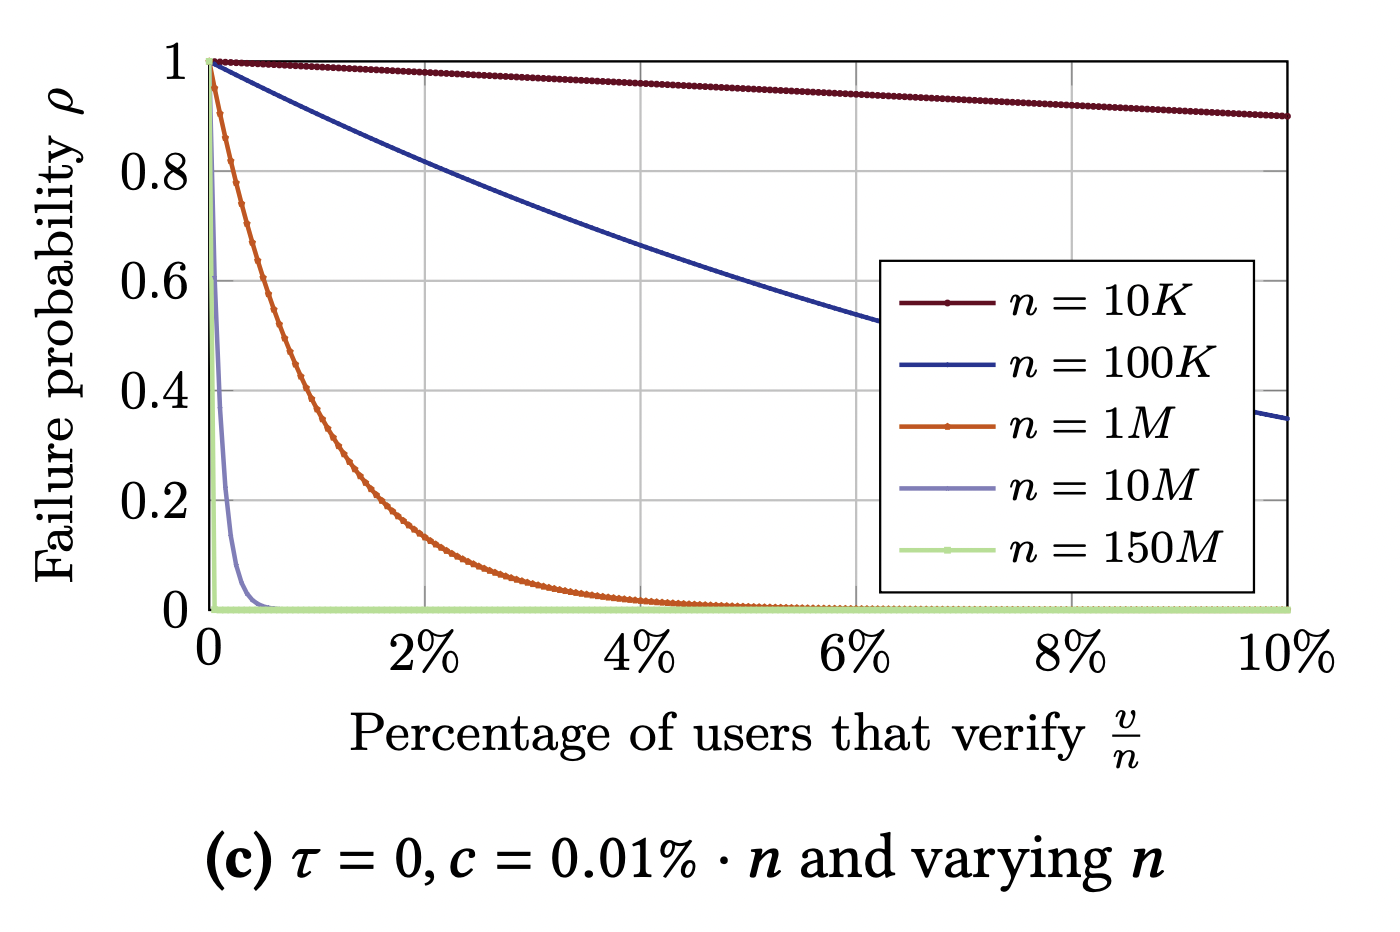
\includegraphics[width=130mm]{FailureProbability.png}
   \caption{Failure Probability \cite{GP21}}
   \label{overflow}
   \end{figure}


Now, lets evaluate the failure probability if we are using folding.
In the initial round, with no changes, the failure probability for 20k users remains at $13\%$.


\begin{figure}[H]
   \centering
   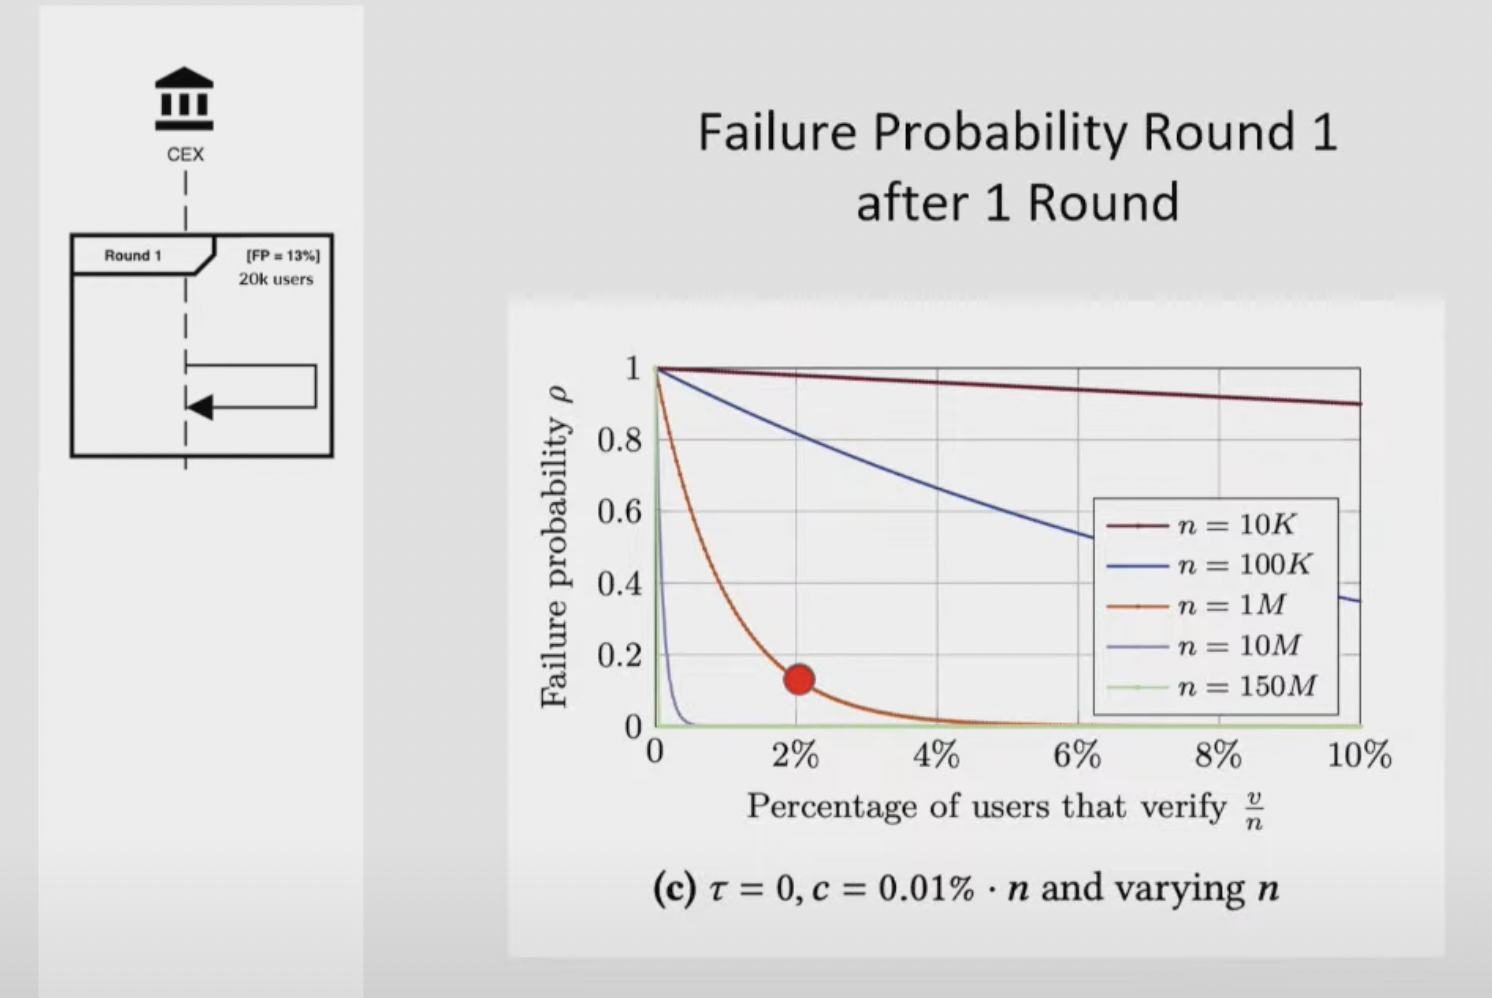
\includegraphics[width=130mm]{FailureProbabilityRound1.png}
   \caption{Failure Probability Round 1 \cite{NS23}}
   \label{overflow}
   \end{figure}


However, if we have 20k distinct users in round 2, the failure probability of round 1 decreases to $1.6\%$ .


\begin{figure}[H]
   \centering
   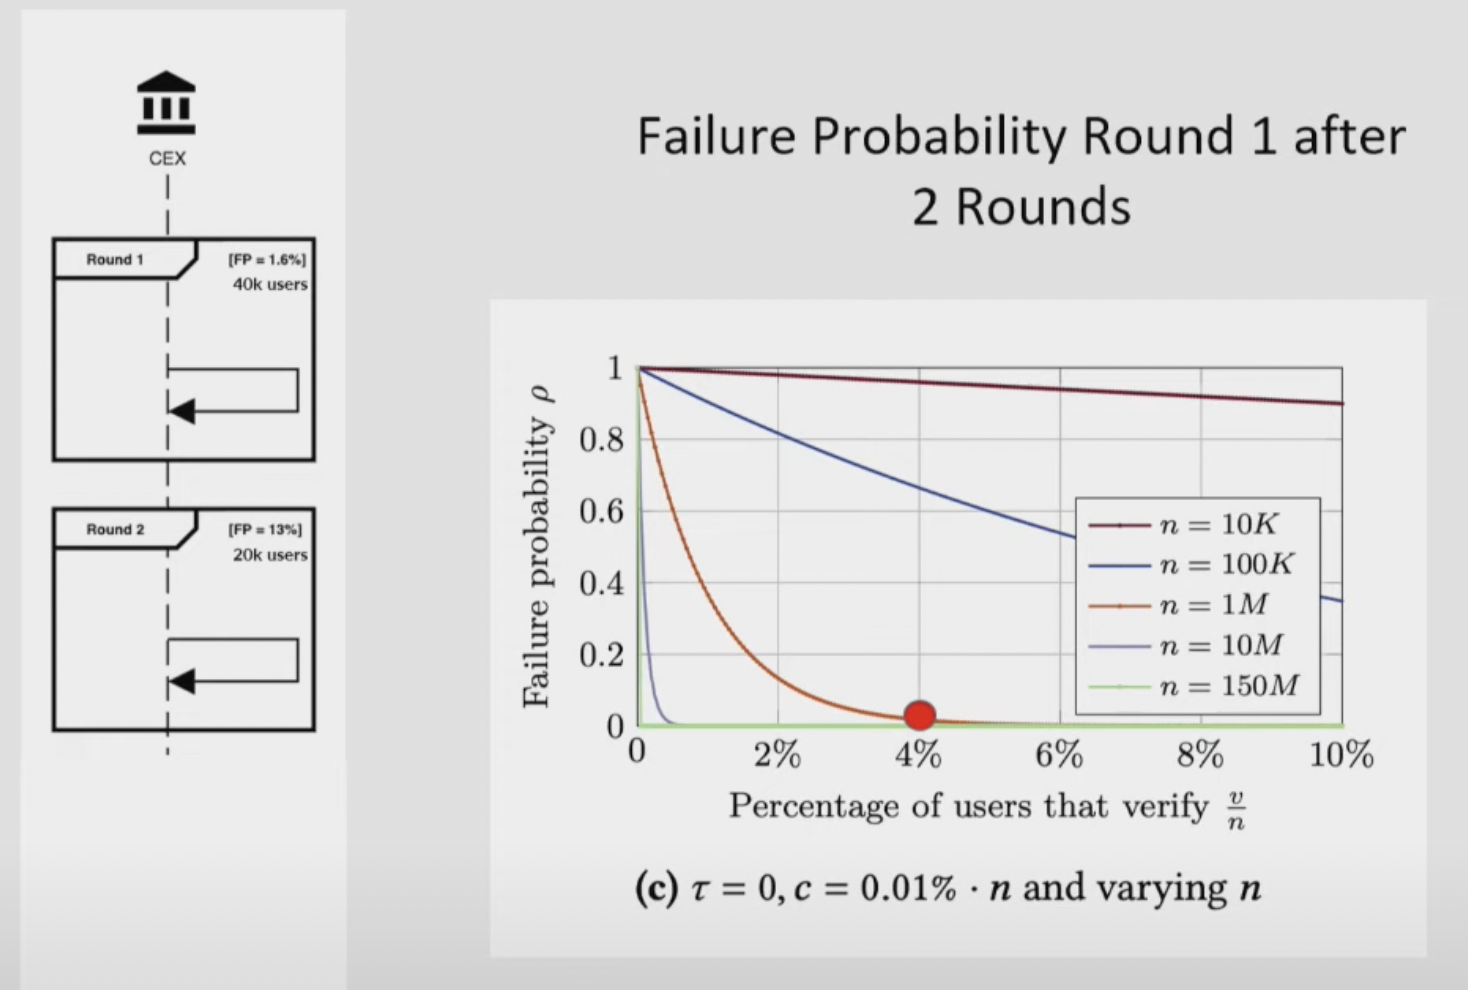
\includegraphics[width=130mm]{FailureProbabilityRound2.png}
   \caption{Failure Probability Round 1 After 2 Rounds\cite{NS23}}
   \label{overflow}
   \end{figure}


If we have 20k different users in round 3, the failure probability of round 1 further decreases to $0.2\%$ .


\begin{figure}[H]
   \centering
   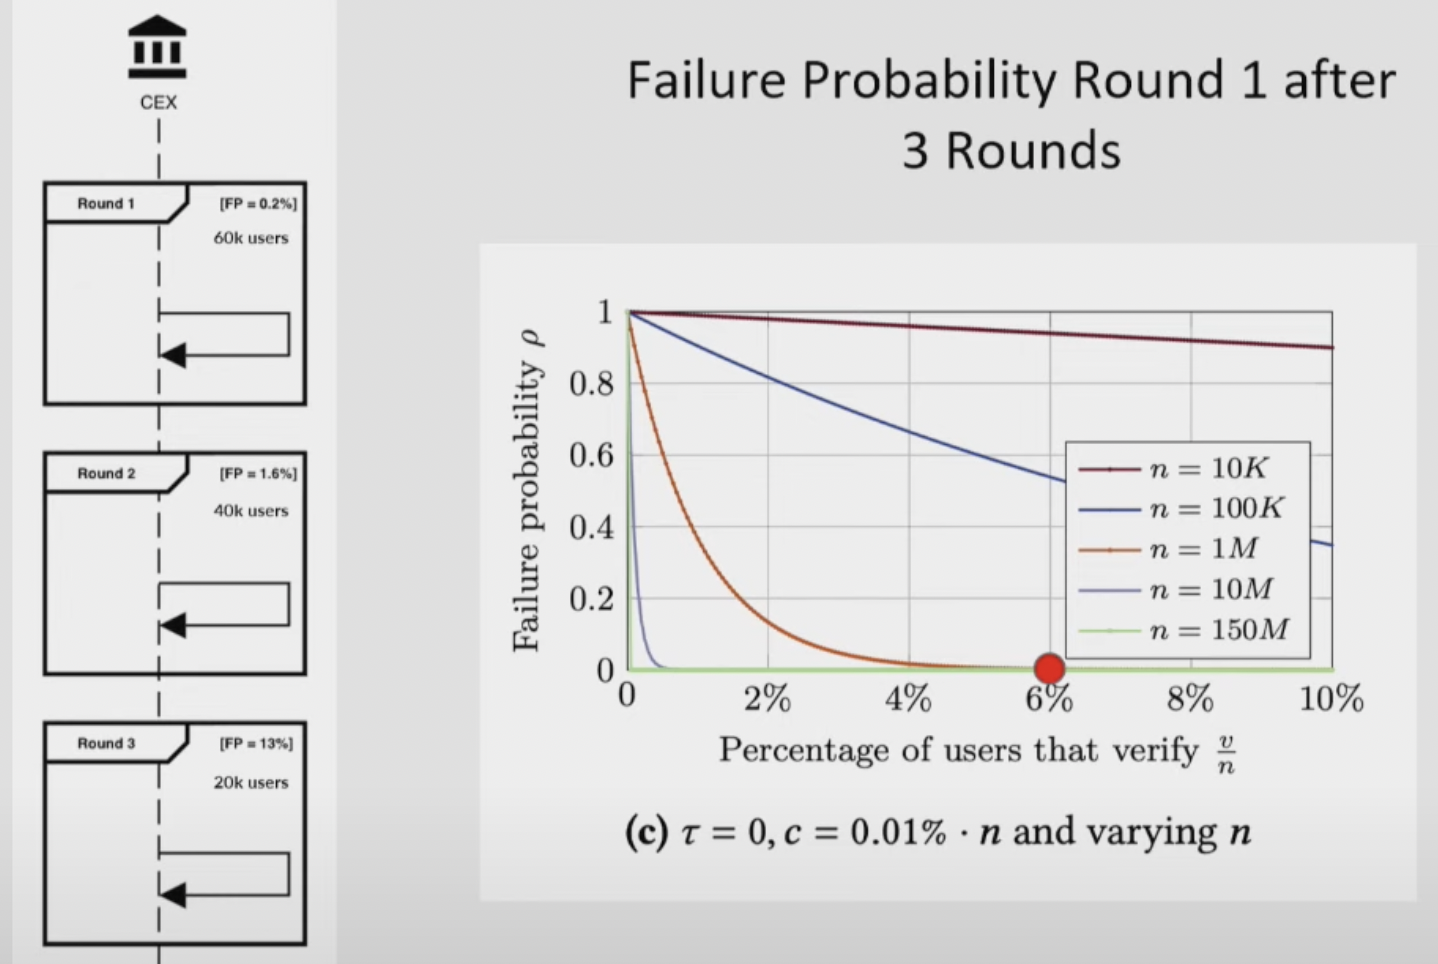
\includegraphics[width=130mm]{FailureProbabilityRound3.png}
   \caption{Failure Probability Round 1 after 3 Rounds \cite{NS23}}
   \label{overflow}
   \end{figure}
The key takeaway here is that without folding, you require $4\%$ of users to verify every round. However, with folding you only need
$4\%$  of users to participate in at least 1 round. This significantly reduces the burden on the user to verify, while increasing the confidence in the proof.


\subsection{Circuit Design}
The private inputs vary for each instance, whereas the public inputs are carried over from round to round.
In order to implement folding, we need to slightly adjust our \hyperref[subsec:pi]{circuit}. While most of the circuit stays the same, we change the way we handle inputs and outputs.
The private inputs vary for every instance, while the public inputs are carried over from round to round.
\begin{figure}[H]
   \centering
   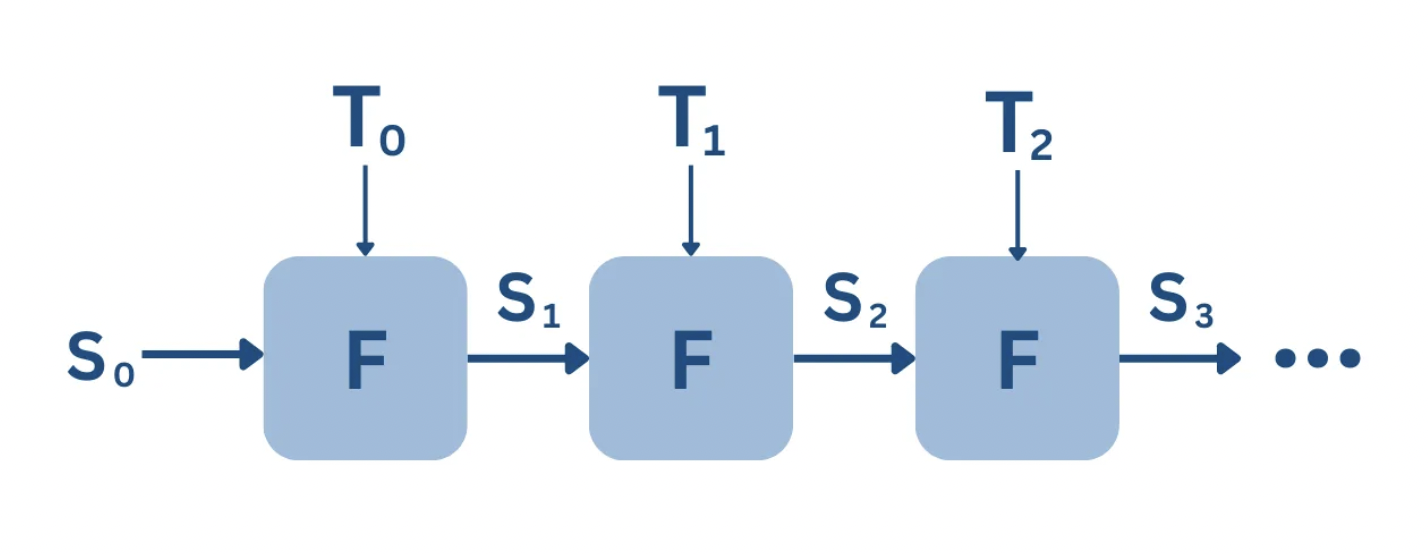
\includegraphics[width=130mm]{FoldingCircuit.png}
   \caption{Folding \cite{VRS23}}
   \label{overflow}
   \end{figure}
In this chart, S represent the public input and output, which is passed around from round to round. F is the round, while T is the private input.
We define S as $step_in$ and $step_out$ within our circuit.


\paragraph{Inputs}
\begin{itemize}


   \item List of neighbors sum (private)
  
   \item List of neighbors hash (private)


   \item List of neighbors binary (private)


   \item Root hash (private)


   \item Root sum (private)


   \item User balance (private)


   \item User email hash (private)


   \item Steps in (public)
  
   \end{itemize}


\paragraph{Outputs}
\begin{itemize}
   \item Steps out (public)
   \end{itemize}


\paragraph{Steps}
\begin{itemize}
   \item Balance included
   \item Root sum
   \item Root hash
   \item User balance
   \item User email hash
   \end{itemize}
These steps encompass all the public values we initially had in the circuit.
None of the variables of the steps are used in the circuit itself. They are used as a means to make a value public.
The steps are all the public values we had in the first circuit.


The initial circuit takes meaningless values as inputs, while the following circuits take the public values of the previous circuit.
At the end you only have to verify a single proof. You also need to compare the circuit output with the proof of liabilities outputs for every round.


%Mina proof of recursion
%summa
%https://summa.gitbook.io/summa/v/1/circuits/merkle-sum-tree-inclusion
%https://www.youtube.com/watch?v=sRAA1RYYHEs
%https://hackmd.io/@summa/HkGMF4Ovn#The-problem